\documentclass{article}
\usepackage{graphicx}
\usepackage{graphicx} 
\usepackage{amssymb}
\usepackage{float}
\usepackage{amsmath}
\usepackage{algorithm}
\usepackage{algpseudocode}

\title{Linear Classifiers}
\author{ }
\date{ }

\begin{document}
	
	\maketitle 
	
	A linear classifier is a type of hypothesis for the supervised learning setup. To visualize how linear classifiers work, one must plot all $x$ values in $D_n$ onto the $\mathbb{R}^d$ space. Each axis of the $\mathbb{R}^d$ space (i.e. $x_1$, $x_2$, ... , $x_n$) corresponds to a dimension of the vector $x$. The first dimension of $x$ is its first entry, the second dimension is its second entry, and so on. Some of the plotted points are assigned a $y$ value of $+1$ whereas others are assigned to $-1$.\\
	
    \begin{figure}[H]
        \centering
        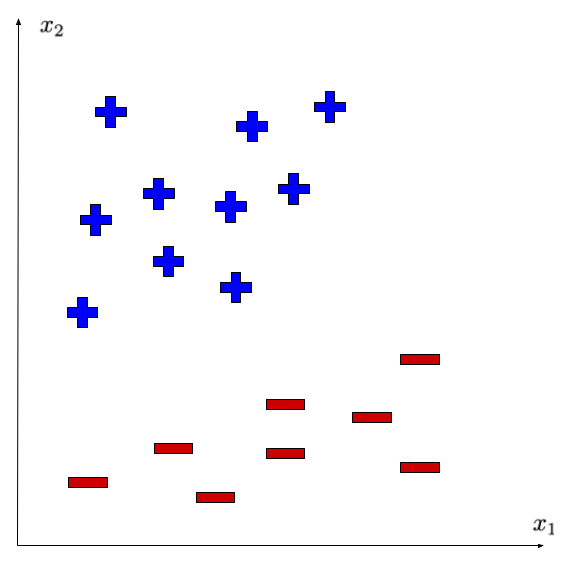
\includegraphics[width=0.5\linewidth]{Plotted X Values.png}
    \end{figure}
	
	Once the dataset is visualized on a graph, how to write a classifier becomes really obvious! For the two dimensional space above, one just needs to draw a line that separates $\mathbb{R}^2$ into a $+1$ subspace and $-1$ subspace. In otherwords, one just needs to find a line such that all points that were assigned $+1$ in the dataset sit on one side while all points that were assigned $-1$ sit on the other side. The separator that does the job is called a linear classifier. \\
	
    \begin{figure}[H]
        \centering
        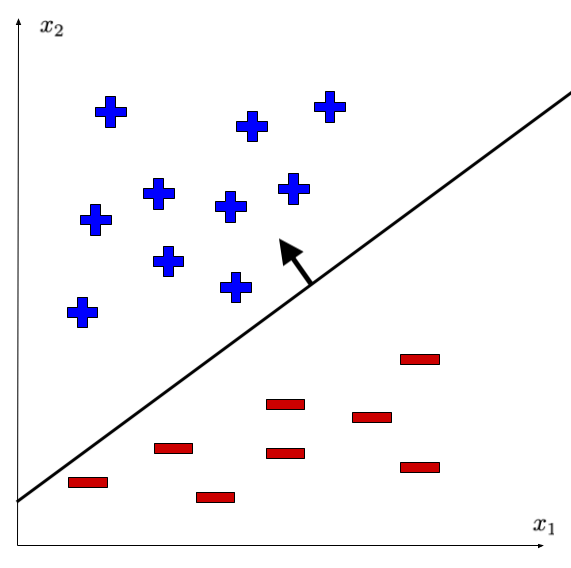
\includegraphics[width=0.5\linewidth]{Classified X Values.png}
    \end{figure}
    		
	For a dataset with two-dimensional $x$ vectors, linear classifiers, as described earlier, are just lines. For a dataset with three-dimensional $x$ vectors, linear classifiers are planes. When the dataset contains $n$-dimensional $x$ vectors, the general term used to describe the separator that classifies them is a hyperplane For the $\mathbb{R}^n$ space, hyperplanes are a space with $n-1$ dimensions. A hyperplane has a normal that points in the direction of the $+1$ subspace. \\
	
	A linear classifier may be written formally as $h(x; \theta, \theta_0)=sign(\theta^T{x}+\theta_0)=\begin{cases}
        +1, \theta^Tx+\theta_0>0\\
        -1, otherwise
    \end{cases}$. Visibly, it has two parameters $\theta$ and $\theta_0$. Learning algorithms try to find the parameters that will construct a separator that accurately classifies $+1$ from $-1$. $\theta \in \mathbb{R}^d$ and $\theta_0\in\mathbb{R}$.  \\

    The simplest learning algorithm that one can begin with is the random linear classifier algorithm. The algorithm works by producing random parameters $k$ times. At the end, it returns the parameters with the lowest training set error. $k$ is called a hyperparameter. It is not a parameter of the hypothesis. Rather, it is a parameter of the learning algorithm. It impacts how training occurs. \\

    \begin{algorithm}
    \begin{algorithmic}[]
        \State \textbf{Input:} $D_n$, $k$
        \For{$j = 1$ to $k$}
            \State $\theta^{(j)} \gets \text{random}(\mathbb{R}^d)$
            \State $\theta^{(j)}_0 \gets \text{random}(\mathbb{R})$
        \EndFor
        \State $j^* \gets \arg\min_{j \in \{1, ..., k\}} {E_n(h(\cdot,\theta,\theta_0))}$ \\
        \Return $\theta^{(j^*)}, \theta_0^{(j^*)}$
    \end{algorithmic}
    \end{algorithm}
    



    
	
\end{document}



























